\documentclass[11pt,a4paper]{article}
\usepackage[T1]{fontenc}
\usepackage[utf8]{inputenc}
\usepackage{lmodern}
\usepackage[margin=22mm,headheight=16pt]{geometry}
\usepackage{amsmath,amssymb,graphicx,array,longtable,booktabs}
\usepackage{microtype,xcolor,hyperref,xurl,fancyhdr}
\definecolor{Navy}{HTML}{17324D}
\definecolor{Teal}{HTML}{087F8C}
\definecolor{Gold}{HTML}{B88128}
\hypersetup{colorlinks=true,linkcolor=Navy,urlcolor=Teal,bookmarksnumbered=true,hypertexnames=false}
\setlength{\parindent}{0pt}
\setlength{\parskip}{6pt}
\setlength{\emergencystretch}{4em}
\setcounter{tocdepth}{1}
\pagestyle{fancy}\fancyhf{}
\fancyfoot[R]{\small\thepage}
\fancyfoot[L]{\small\sffamily Sharif University of Technology}
\renewcommand{\headrulewidth}{0.3pt}
\makeatletter
\renewcommand\section{\@startsection{section}{1}{\z@}{-3.2ex plus -1ex minus -.2ex}{1.6ex plus .2ex}{\normalfont\Large\sffamily\bfseries\color{Navy}}}
\renewcommand\subsection{\@startsection{subsection}{2}{\z@}{-2.5ex plus -1ex minus -.2ex}{1.2ex plus .2ex}{\normalfont\large\sffamily\bfseries\color{Teal}}}
\makeatother
\fancyhead[L]{\small\sffamily\color{Navy}Sharif University of Technology}\fancyhead[R]{\small\sffamily\color{Teal}Project Assignment}\begin{document}
\begin{titlepage}\centering\vspace*{7mm}

\includegraphics[width=31mm]{assets/sharif_emblem_en.png}\par\vspace{5mm}
{\Large\sffamily\bfseries\color{Navy}SHARIF UNIVERSITY OF TECHNOLOGY\par}
\vspace{2mm}{\sffamily Department of Electrical Engineering\par}
\vspace{17mm}{\color{Teal}\rule{\linewidth}{1.4pt}}\par\vspace{6mm}
{\large\sffamily\color{Teal}PROJECT ASSIGNMENT\par}
\vspace{8mm}{\huge\sffamily\bfseries\color{Navy}Periodic Real-Time Scheduling Simulator: RM, DM, and EDF\par}
\vspace{9mm}{\color{Gold}\rule{45mm}{1pt}}\par\vfill
\begin{minipage}{.88\linewidth}
{\sffamily\color{Teal}INSTRUCTOR / INSTRUCTORS}\par
Dr Iman Gholampour\par\vspace{7mm}
{\sffamily\color{Teal}ACADEMIC CONTEXT}\par
Embedded Systems\par\end{minipage}\vfill
\end{titlepage}
\tableofcontents\clearpage
\section{Part 1: theoretical investigation}

Answer each question with a reasoned discussion. Compare single-processor, multicore, and system-on-chip embedded architectures, with benefits, limitations, and application examples. Compare a real-time operating system with general-purpose Linux/\allowbreak{}Windows in scheduling, memory management, interrupt handling, and determinism. Explain priority inversion and compare priority inheritance with priority-ceiling protocols. Distinguish hard and soft real-time requirements and give industrial/\allowbreak{}commercial examples. Discuss reliability and fault tolerance in industrial and automotive embedded systems:\allowbreak{} watchdogs, redundancy, checkpointing, and error-detection codes, including both advantages and limitations. Discuss memory, computation, and energy constraints in TinyML/\allowbreak{}edge AI and explain quantization, pruning, and model compression.

\section{Processor calculations}

Processor A runs at 2 GHz and executes a 12-million-instruction program. Processor B runs at 1.5 GHz and executes a nine-million-instruction program. Use the four category weights and CPI values below. Calculate weighted CPI for both cases, execution time on each processor, and performance in MIPS. State the interpretation of the provided percentages as instruction-mix weights.


\begingroup\small\setlength{\tabcolsep}{3pt}\renewcommand{\arraystretch}{1.2}
\begin{longtable}{@{}p{0.2263\linewidth}p{0.2263\linewidth}p{0.2263\linewidth}p{0.2263\linewidth}@{}}
\toprule
\textbf{Category} & \textbf{Weight (percent)} & \textbf{CPI, case 1} & \textbf{CPI, case 2} \\ \midrule
\endfirsthead
\textbf{Category} & \textbf{Weight (percent)} & \textbf{CPI, case 1} & \textbf{CPI, case 2} \\ \midrule \endhead
1 & 40 & 2 & 3 \\
2 & 30 & 3 & 2 \\
3 & 10 & 4 & 3 \\
4 & 20 & 5 & 4 \\
\bottomrule\end{longtable}\endgroup
\begingroup\small\setlength{\tabcolsep}{3pt}\renewcommand{\arraystretch}{1.18}\begin{longtable}{@{}p{0.2200\linewidth}p{0.2200\linewidth}p{0.2200\linewidth}p{0.2200\linewidth}@{}}
\caption{Processor calculations - numerical data and parameters.}\label{tab:012_p004_table10}\\\toprule
\textbf{Task} & \textbf{Assigned frequency (\%)} & \textbf{CPI:\allowbreak{} case 1} & \textbf{CPI:\allowbreak{} case 2} \\ \midrule\endfirsthead \textbf{Task} & \textbf{Assigned frequency (\%)} & \textbf{CPI:\allowbreak{} case 1} & \textbf{CPI:\allowbreak{} case 2} \\ \midrule\endhead
1 & 40 & 2 & 3 \\
2 & 30 & 3 & 2 \\
3 & 10 & 4 & 3 \\
4 & 20 & 5 & 4 \\
\bottomrule\end{longtable}\endgroup
\begin{figure}[!htbp]\centering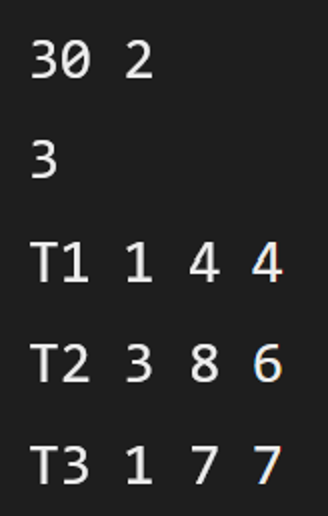
\includegraphics[width=\linewidth,height=.72\textheight,keepaspectratio]{assets/012_p005_01.png}\caption{Diagram or recorded result: Processor calculations.}\label{fig:012_p005_010}\end{figure}
\begin{figure}[!htbp]\centering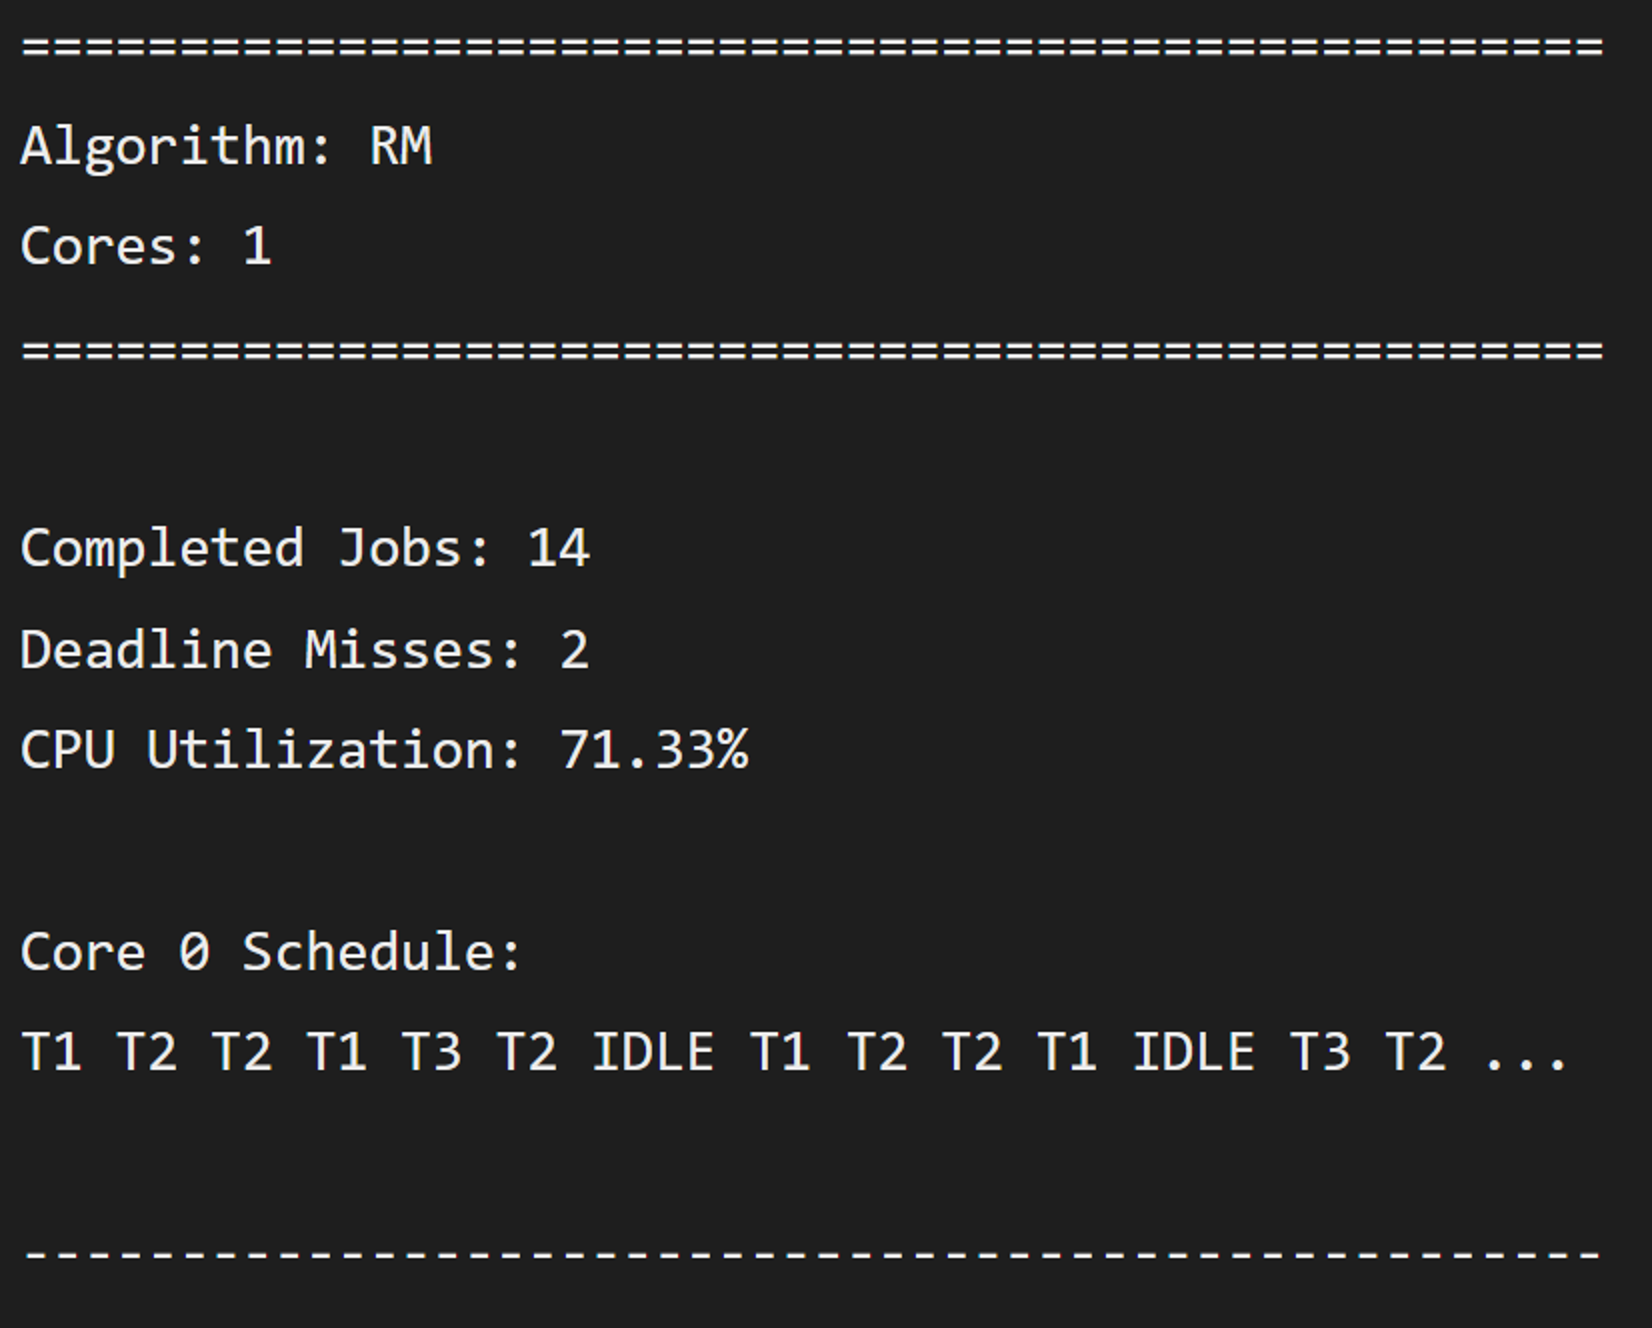
\includegraphics[width=\linewidth,height=.72\textheight,keepaspectratio]{assets/012_p006_01.png}\caption{Diagram or recorded result: Processor calculations.}\label{fig:012_p006_010}\end{figure}
\begin{figure}[!htbp]\centering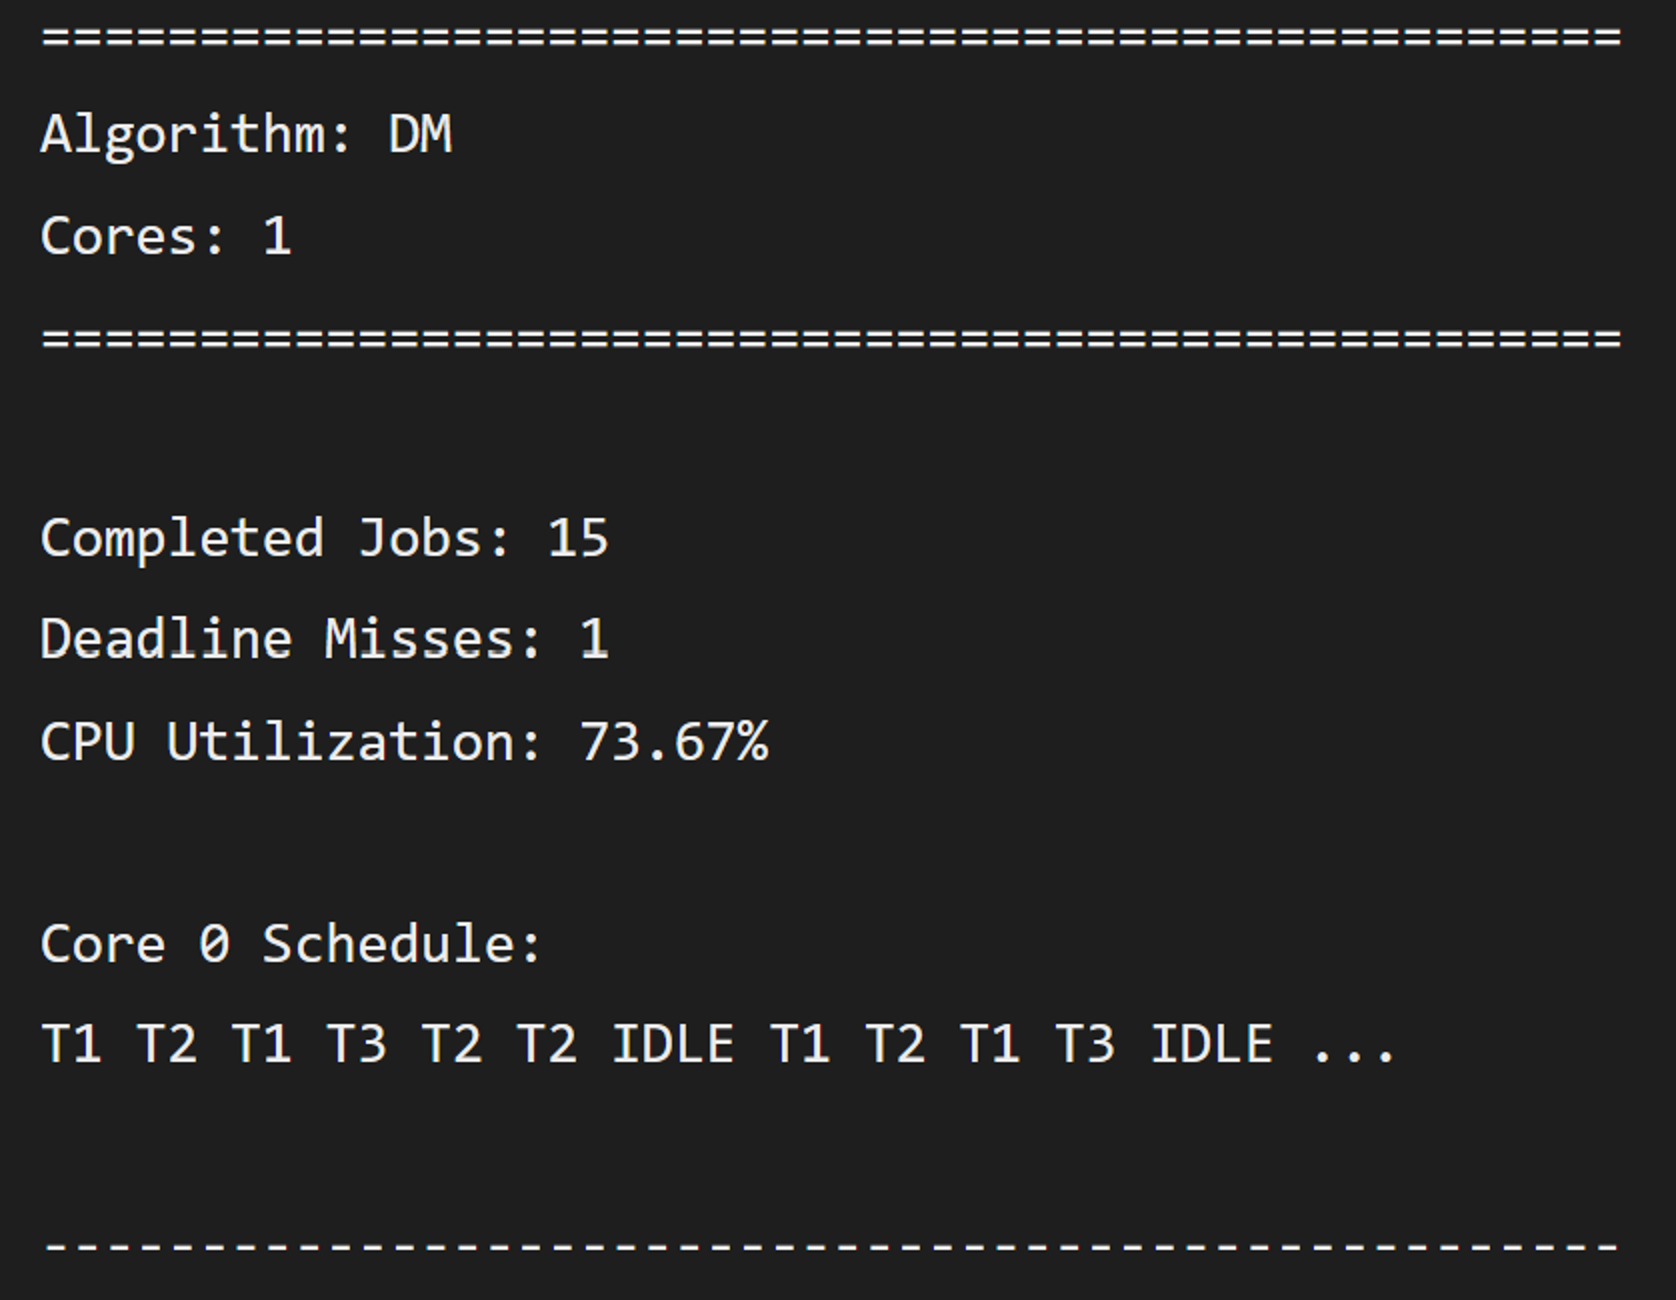
\includegraphics[width=\linewidth,height=.72\textheight,keepaspectratio]{assets/012_p006_02.png}\caption{Diagram or recorded result: Processor calculations.}\label{fig:012_p006_020}\end{figure}
\begin{figure}[!htbp]\centering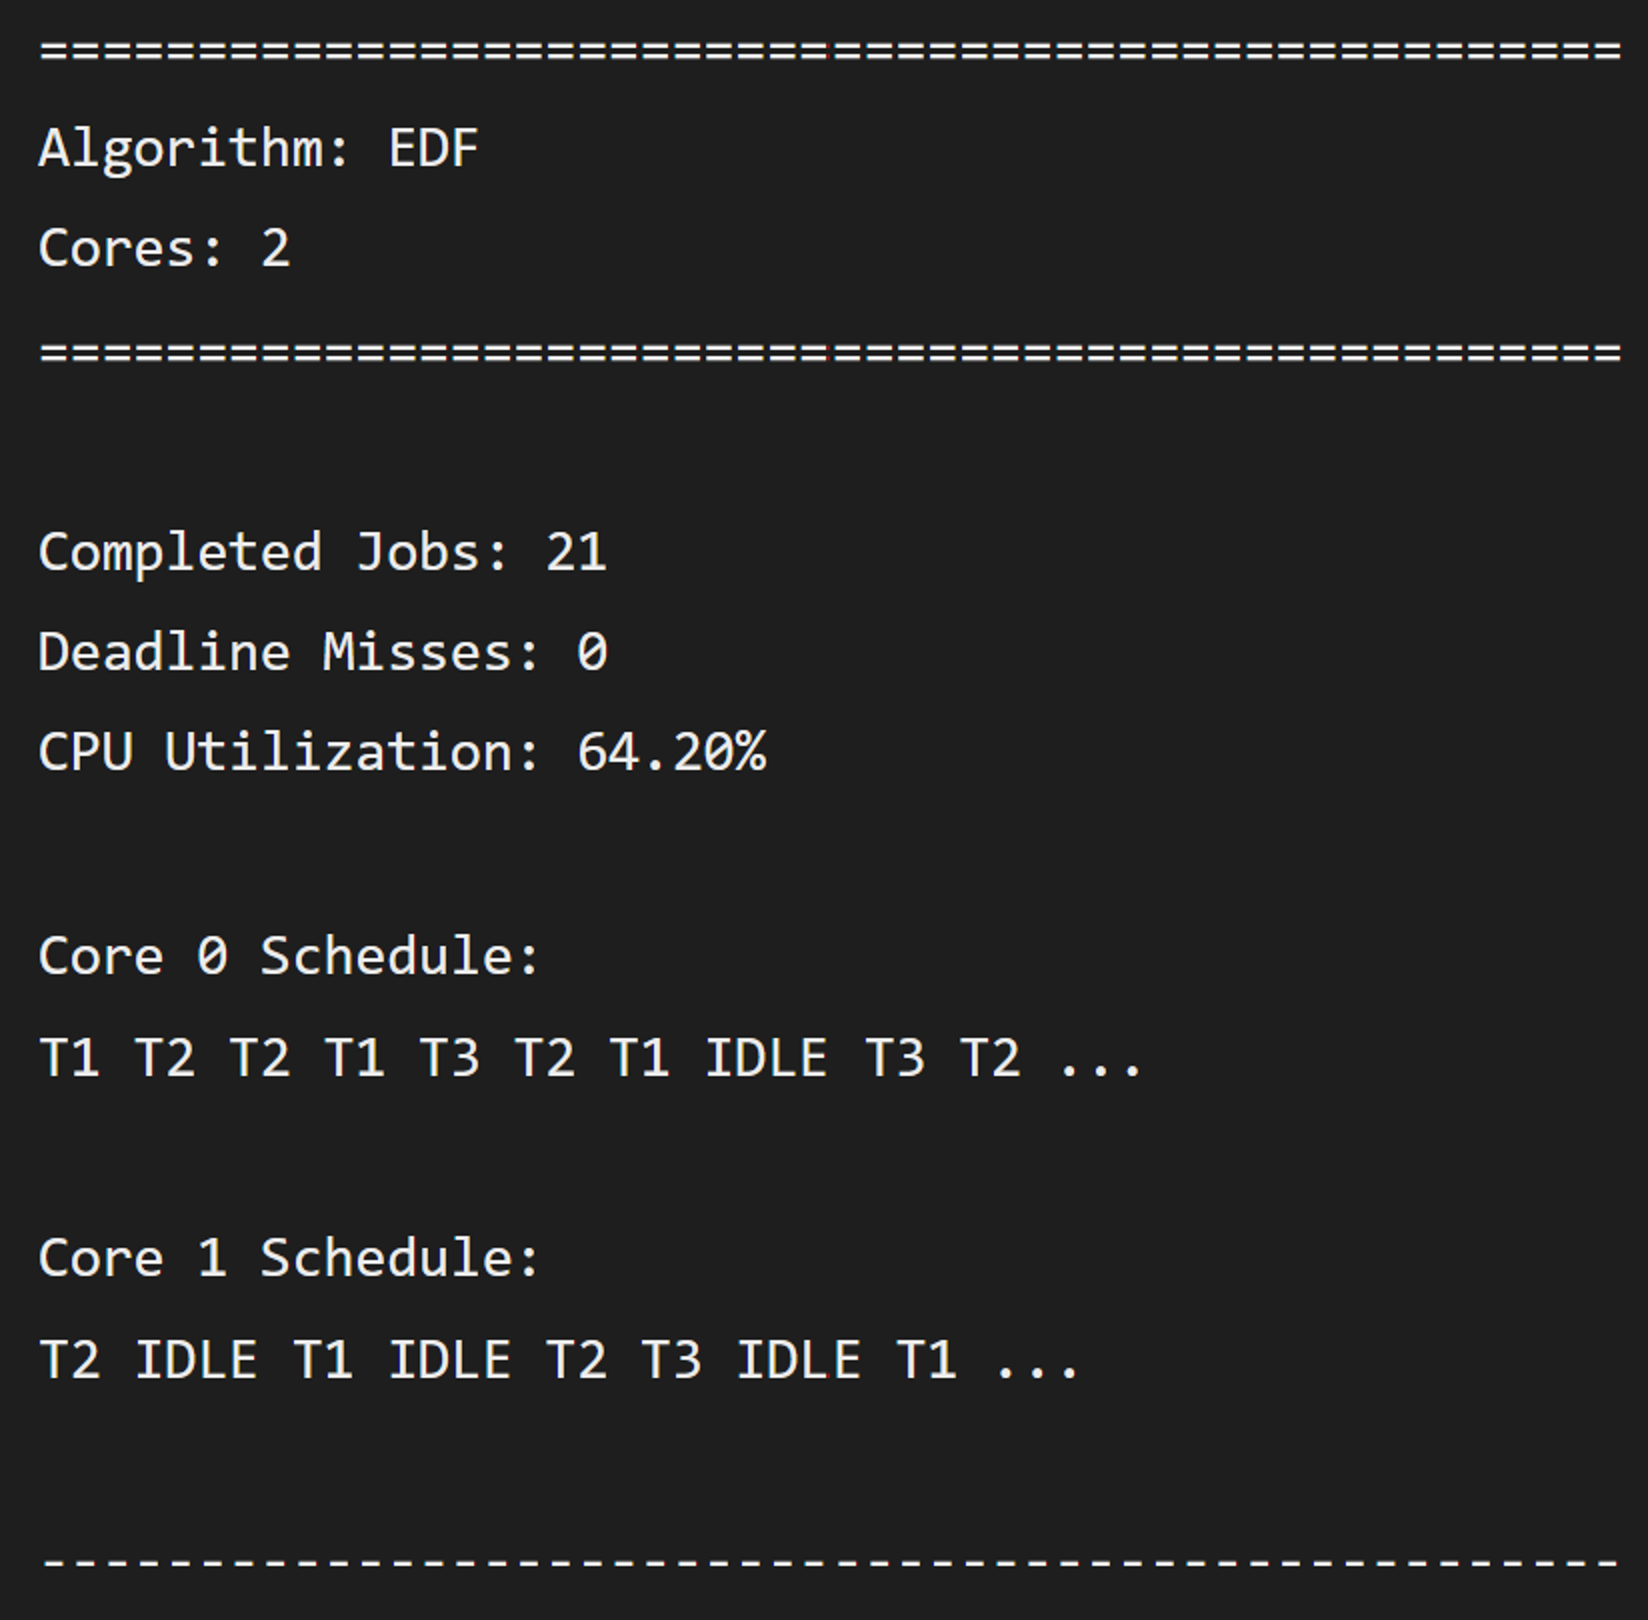
\includegraphics[width=\linewidth,height=.72\textheight,keepaspectratio]{assets/012_p006_03.png}\caption{Diagram or recorded result: Processor calculations.}\label{fig:012_p006_030}\end{figure}
\clearpage
\section{Part 2: scheduling implementation}

Implement a stepwise simulation of periodic tasks, each described by execution time C, period T, and relative deadline D. Implement Rate Monotonic, Deadline Monotonic, and Earliest Deadline First for one core. Extend the simulator to two cores with a shared ready queue, permitting simultaneous execution of distinct jobs. Compare completed jobs, deadline misses, and utilization. Read input.txt:\allowbreak{} the first line specifies simulation duration and core count;\allowbreak{} the second gives the number of tasks;\allowbreak{} later lines give name, execution time, period, and relative deadline. Write a text output for each algorithm containing algorithm name, core count, completed-job count, misses, utilization, and each core's time schedule. Produce a separate Gantt chart for each algorithm/\allowbreak{}core configuration, with consistent colors for each task. Analyze differences in utilization and missed deadlines, the circumstances under which EDF can behave better, and the effect of extra cores. Submit Python source, input, text output, report, and plots.

\begin{figure}[!htbp]\centering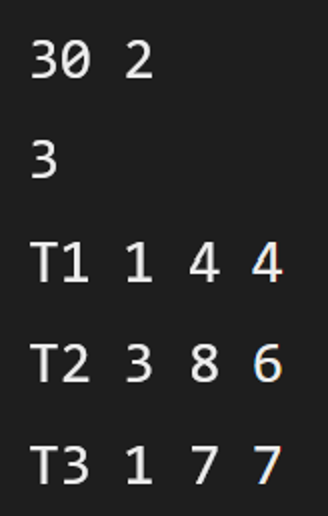
\includegraphics[width=\linewidth,height=.72\textheight,keepaspectratio]{assets/012_p007_01.png}\caption{Diagram or recorded result: Part 2: scheduling implementation.}\label{fig:012_p007_010}\end{figure}
\begin{figure}[!htbp]\centering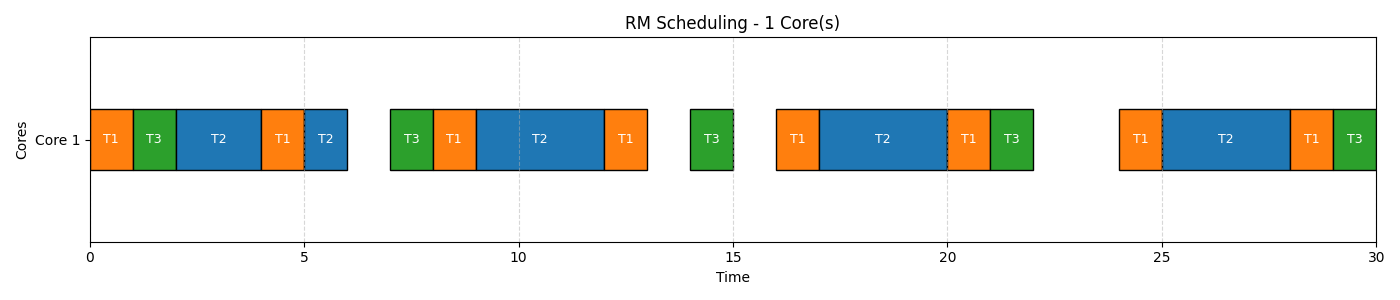
\includegraphics[width=\linewidth,height=.72\textheight,keepaspectratio]{assets/012_p007_02.png}\caption{Diagram or recorded result: Part 2: scheduling implementation.}\label{fig:012_p007_020}\end{figure}
\begin{figure}[!htbp]\centering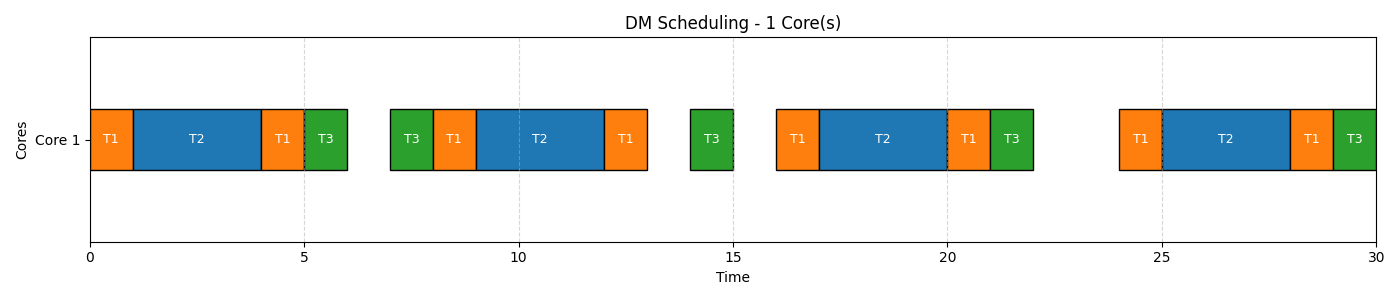
\includegraphics[width=\linewidth,height=.72\textheight,keepaspectratio]{assets/012_p007_03.png}\caption{Diagram or recorded result: Part 2: scheduling implementation.}\label{fig:012_p007_030}\end{figure}
\begin{figure}[!htbp]\centering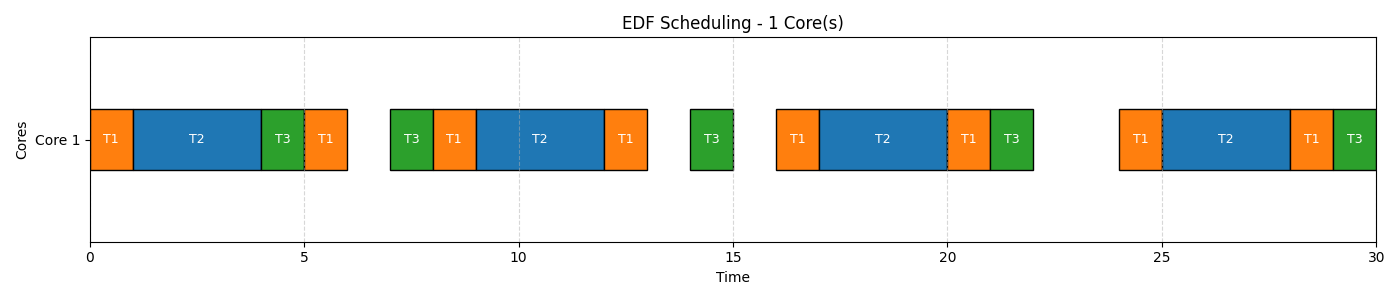
\includegraphics[width=\linewidth,height=.72\textheight,keepaspectratio]{assets/012_p007_04.png}\caption{Diagram or recorded result: Part 2: scheduling implementation.}\label{fig:012_p007_040}\end{figure}
\begin{figure}[!htbp]\centering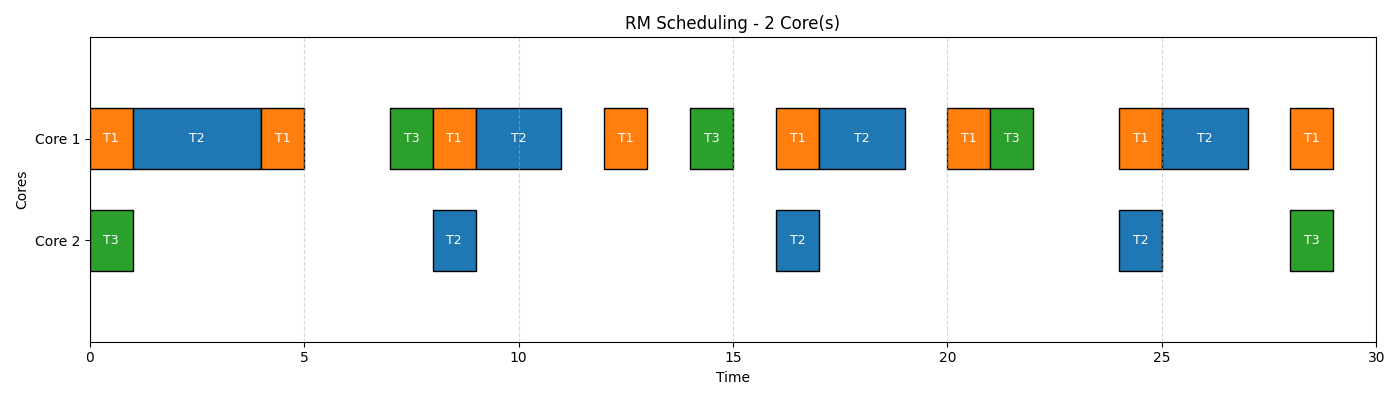
\includegraphics[width=\linewidth,height=.72\textheight,keepaspectratio]{assets/012_p008_01.png}\caption{Diagram or recorded result: Part 2: scheduling implementation.}\label{fig:012_p008_010}\end{figure}
\begin{figure}[!htbp]\centering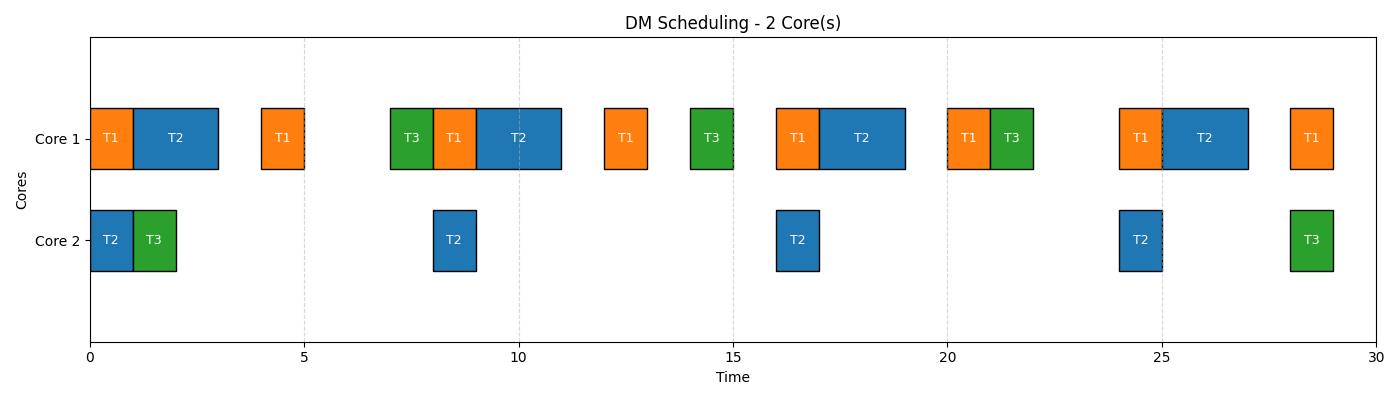
\includegraphics[width=\linewidth,height=.72\textheight,keepaspectratio]{assets/012_p008_02.png}\caption{Diagram or recorded result: Part 2: scheduling implementation.}\label{fig:012_p008_020}\end{figure}
\begin{figure}[!htbp]\centering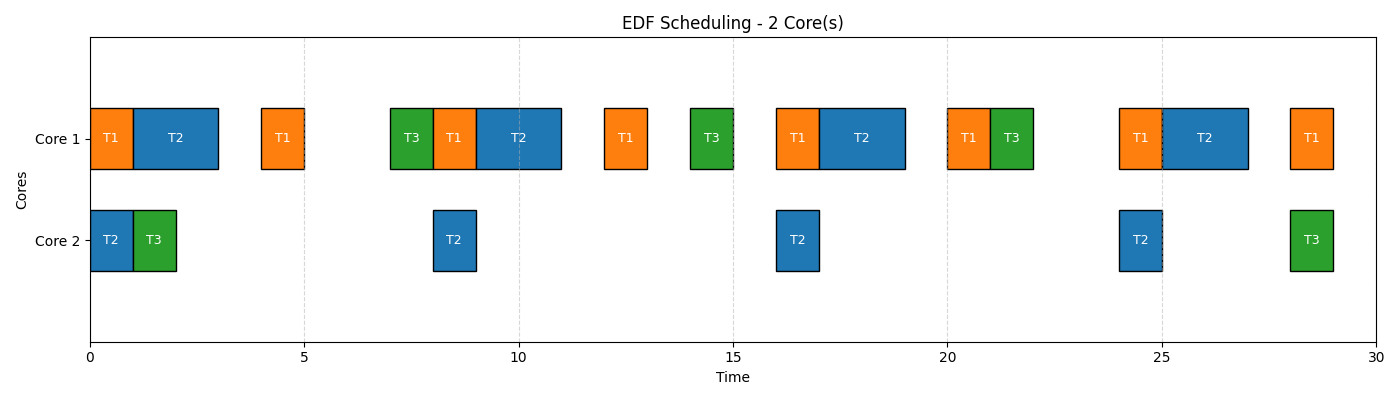
\includegraphics[width=\linewidth,height=.72\textheight,keepaspectratio]{assets/012_p008_03.png}\caption{Diagram or recorded result: Part 2: scheduling implementation.}\label{fig:012_p008_030}\end{figure}
\clearpage
\end{document}